\section{Minimization w/ Inequality Constraints}

\begin{frame}{Three families you should know (high level)}
\textbf{Goal:} Handle inequalities $c(x)\ge 0$ (and equalities) robustly and efficiently.

\medskip
\textbf{Families.}
\begin{enumerate}
\item \textbf{Penalty}: embed violations in the objective; crank a parameter $\rho\uparrow$.
\item \textbf{Augmented Lagrangian (ALM)}: maintain multipliers \& a \emph{moderate} penalty; solve easier subproblems.
\item \textbf{Interior-Point (PDIP)}: enforce $c(x)>0$ via a barrier; follow the \emph{central path} with primal--dual Newton.
\end{enumerate}

\textbf{Rule of thumb.} Penalty is simplest; ALM is a strong default for medium accuracy; PDIP is the gold standard for convex QPs and very robust with Newton. 
\end{frame}




\begin{frame}{Inequality-Constrained Minimization}
\textbf{Problem Setup:}
$$
\min f(x) \quad \text{s.t. } c(x) \geq 0
$$
\textbf{KKT conditions:} 

$$
\nabla f - \left(\frac{\partial c(x)}{\partial x}\right)^T \lambda = 0 \quad \text{(stationarity)}
$$

$$
c(x) \geq 0 \quad \text{(primal feasibility)} \quad \quad \quad  \lambda \geq 0 \quad \text{(dual feasibility)}
$$ 

$$
\lambda \circ c(x) = \lambda^T c(x) = 0 \quad \text{(complementarity)}
$$

\textbf{Unlike equality case, we can’t directly solve KKT conditions with Newton! Why?}

 
\end{frame}


\begin{frame}{Lots of solution methods to use: Active Set Method} 
\underline{\textbf{Active Set Method}}
\begin{itemize}
    \item High level idea: Guess which inequalities are redundant at optimality and throw them away.
    \item Switch inequality constraints on/off in outer-loop and solve equality-constrained problem.
    \item Works well if you can guess active set well ( common in MPC where good warm-starts are common).
    \item Has really bad worst-time complexity.
    \item Usually custom heuristics are used for specific problem classes/structure.

\end{itemize}
\end{frame}

% --- Slide 1: Idea & Algorithm ---------------------------------------------
\begin{frame}{Penalty Methods: Idea \& Algorithm}
\underline{\textbf{Penalty Method}}: Replace constraints with cost terms that penalize violation!
\[
\min_x\; f(x) \;+\; \tfrac{\rho}{2}\,\big\|c^-(x)\big\|_2^2,\qquad
c^-(x):=\min(0,c(x))\ \text{(elementwise)}.
\]

\textbf{Algorithm sketch.}
\begin{enumerate}
\item Start with a small $\rho>0$; minimize the penalized unconstrained objective.
\item Increase $\rho$ (e.g., $\times 10$) and warm start from previous $x$.
\item Stop when $c^-(x)$ is small enough.
\end{enumerate}
\end{frame}


% --- Slide 3: Quadratic penalty & why large $\rho$ is needed ----------------
\begin{frame}{Quadratic penalty: need large $\rho$ for strong feasibility pressure}
\begin{columns}[T,onlytextwidth]
\column{0.45\textwidth}
\small
\textbf{Pros.} Dead simple; reuse unconstrained machinery (Grad/Newton + line search). \\
\textbf{Cons.} Ill-conditioning as $\rho\to\infty$; struggles to reach high accuracy; multipliers are implicit. \\
\textbf{Popular fix.} Estimate $\lambda$ (Augmented Lagrangian / ADMM) to converge with finite $\rho$.

\vspace{0.6em}
\textbf{Takeaway.} The penalty outside the feasible set ($x<0$ here) is only quadratic,
so to make violations tiny you often must crank $\rho$ very large $\Rightarrow$ poor conditioning.

\column{0.53\textwidth}
\centering
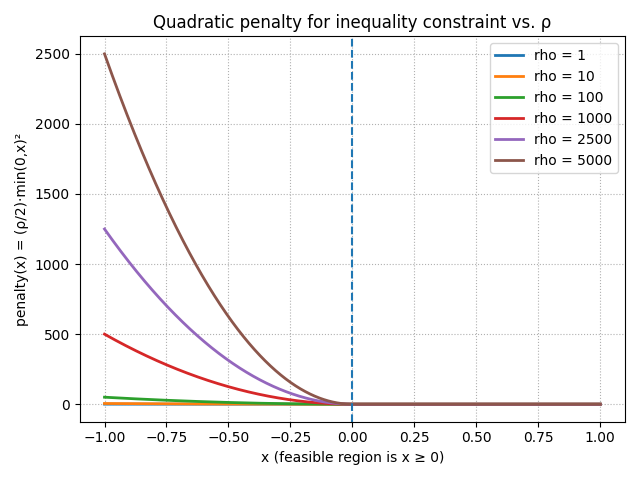
\includegraphics[width=\textwidth]{figures/quadratic_penalty.png}
\end{columns}
\end{frame}







% ---- ALM ---- 
\begin{frame}[t]{Augmented Lagrangian (ALM): fix penalty’s weaknesses}
\setbeamercovered{invisible}

\uncover<1->{\textbf{Core idea.}\; Introduce multipliers $\lambda$ so we can keep $\rho$ moderate and still achieve accuracy.}
 
\uncover<2->{\textbf{Lagrangian for equality case:}\;
$\displaystyle \mathcal{L}_\rho(x,\lambda)=f(x)+\lambda^{\!T}C(x)+\tfrac{\rho}{2}\|C(x)\|_2^2.$}
 
\uncover<3->{\textbf{Outer loop.}
\begin{enumerate}
  \item $x^{k+1}\approx \arg\min_x \mathcal{L}_\rho(x,\lambda^k)$ (unconstrained solve).
  \item $\lambda^{k+1}=\lambda^k+\rho\,C(x^{k+1})$.
\end{enumerate}
}
 
\uncover<4->{\textbf{Inequalities (sketch).}\; Apply to the \emph{hinge} $c^-(x)$ and keep $\lambda\ge 0$:
\[
\mathcal{L}_\rho(x,\lambda)=f(x)-\lambda^{\!T}c(x)+\tfrac{\rho}{2}\|c^-(x)\|_2^2,\quad
\lambda^{k+1}=\max\!\big(0,\lambda^k-\rho\,c(x^{k+1})\big).
\]
}

\uncover<5->{\textbf{Why it works.}\; Subproblems are better conditioned than pure penalty; $\lambda$ estimates improve the model; finite $\rho$ can reach high accuracy.}
\end{frame}




\begin{frame}{ALM in practice (optimization loop view)}
\textbf{Inner solver.} Use (damped) Newton or quasi-Newton on $\mathcal{L}_\rho(\cdot,\lambda^k)$ with Armijo/Wolfe line search. \\
\textbf{Tuning.}
\begin{itemize}
\item Keep $\rho$ fixed or adapt slowly (increase if feasibility stalls).
\item Scale constraints; monitor $|C(x)|$ and stationarity.
\end{itemize}
\textbf{When to pick ALM.}
\begin{itemize}
\item Nonconvex NLPs where feasibility progress matters and you want robust globalization.
\item When medium accuracy is tolerable/fine, or as a precursor to a polished PDIP phase on a convex QP.
\end{itemize}

\end{frame}









\begin{frame}{Interior-Point / Barrier Methods}
\underline{\textbf{TLDR: }} Replace inequalities with barrier function in objective:

$$
\min f(x), \quad x \geq 0 \quad \to \quad \min f(x) - \rho \log(x)
$$

\begin{itemize} 
    \item Gold standard for convex problems.
    \item Fast convergence with Newton and strong theoretical properties.
    \item Used in IPOPT.
\end{itemize} 
\end{frame}


% --- Slide 2: Barrier intuition (contrast) ---------------------------------
\begin{frame}{Barrier intuition issue: $-\log(x)$ blows up near the boundary}
\centering
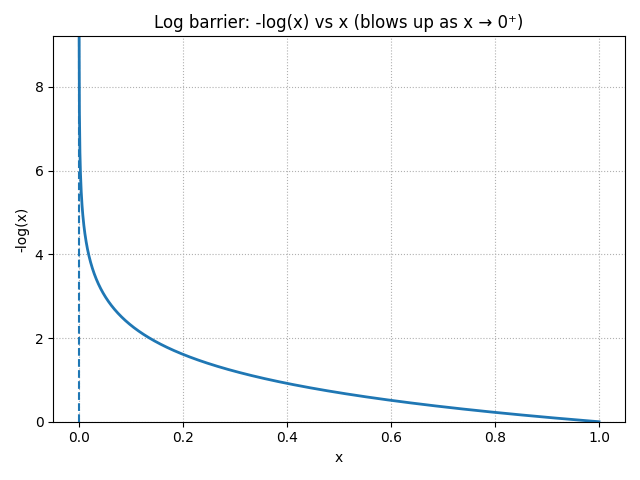
\includegraphics[scale=0.5]{figures/log_barrier.png}
 
{\small
For an inequality like $x\ge 0$, the log barrier $-\log(x)$ goes to $\infty$ as $x\to 0^+$,
creating a \emph{hard wall} at the boundary (contrast with quadratic penalties).
}
\end{frame}



\begin{frame}{Primal-Dual Interior Point Method}
$$
\min f(x) \quad \text{s.t. } x \geq 0
$$

$$
\to \min f(x) - \rho \log(x)
$$

$$
\frac{\partial f}{\partial x} - \frac{\rho}{x} = 0
$$

\begin{itemize}
    \item This “primal” FON condition blows up as $x \to 0$.
    \item We can fix this with the “primal-dual trick.”
\end{itemize}
\end{frame}  


\begin{frame}{The Primal-Dual Trick for IPM}
Introduce new variable $\lambda = \frac{\rho}{x} \quad \Rightarrow \quad x \lambda = \rho$.

$$
\begin{cases}
\nabla f - \lambda = 0 \\
x \lambda = \rho
\end{cases}
$$


\begin{itemize}
    \item This can actually be viewed as a relaxed complementarity slackness from KKT!
    \item Converges to exact KKT solution as $\rho \to 0$.
    \item We lower $\rho$ gradually as solver converges (from $\rho \sim 1$ to $\rho \sim 10^{-6}$).
    \item Note: we still need to enforce $x \geq 0$ and $\lambda \geq 0$ (with line search).
\end{itemize} 
\textbf{We will use another approach from 2022 from a researcher at TRI that developped an even cooler trick.}
    
\end{frame}

\begin{frame}{Log-Domain Interior-Point Method}
\begin{center}
    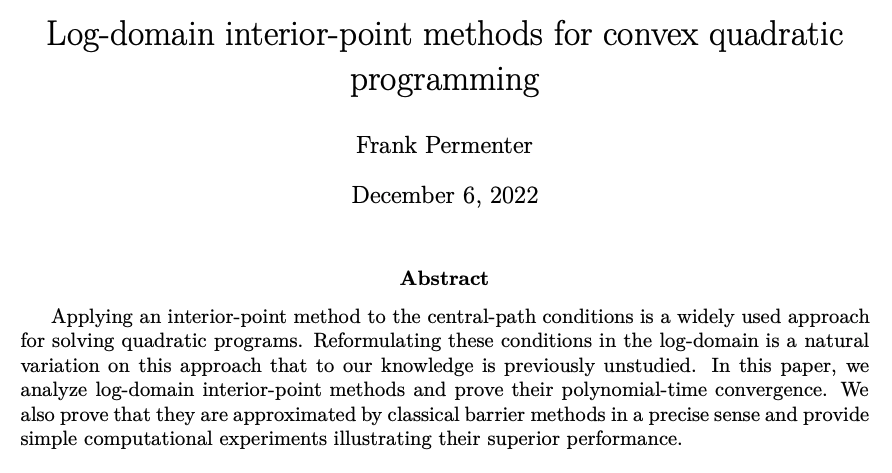
\includegraphics[scale=0.4]{figures/tri_paper.png}
\end{center}
\end{frame}


\begin{frame}{Log-Domain Interior-Point Method}
\textbf{More general constraint case}:   \quad \quad \quad \quad \quad  $\min f(x) \quad \text{s.t. } c(x) \geq 0$

\textbf{Simplify by introducing a “slack variable”:}

$$
\min_{x,s} f(x) \quad \text{s.t. } c(x) - s = 0, \; s \geq 0
$$

$$
\to \min_{x,s} f(x) - \rho \log(s)  \quad \text{s.t. } c(x) - s = 0
$$

\textbf{ Write out Lagrangian:} \quad \quad \quad $L(x,s,\lambda) = f(x) - \rho \log(s) - \lambda^T(c(x)-s)$  
\end{frame}


\begin{frame}{Log-Domain Interior-Point Method}
\textbf{Apply F.O.N.C to Lagrangian from last slide:}

$$
\nabla_x L = \nabla f - \left(\frac{\partial c}{\partial x}\right)^T \lambda = 0
$$

$$
\nabla_s L = \frac{\rho}{s} + \lambda = 0 \quad \Rightarrow \quad s \lambda = \rho
$$

$$
\nabla_\lambda L = s - c(x) = 0
$$

This second equation has a really nice interpretation: relaxed complementarity slackness


\end{frame}





\begin{frame}{Log-Domain Interior-Point Method}

\textbf{Change of variables (elementwise):}
\[
\boxed{\ \rho := s \circ \lambda,\qquad 
\sigma := \tfrac{1}{2}\big(\log s - \log \lambda\big)\ }
\quad\Longleftrightarrow\quad
\boxed{\ s = \sqrt{\rho}\, \circ e^{\sigma},\quad 
\lambda = \sqrt{\rho}\, \circ e^{-\sigma}\ }
\]
{\footnotesize
Here \(\circ\) is the Hadamard (elementwise) product; \(s,\lambda,\rho,\sigma\in\mathbb{R}^m\) with \(s>0,\lambda>0\).
By construction \(s\ge 0,\ \lambda\ge 0\) and \(\rho = s\circ\lambda\) (the relaxed complementarity) holds.}

\vspace{0.6em}

\textbf{KKT (first-order) residuals with inequality \(c(x) - s = 0\):}
\[
r_x(x,\sigma) := \nabla f(x) - J(x)^{\!T}\lambda(\sigma), 
\qquad
r_c(x,\sigma) := c(x) - s(\sigma) = 0,
\]
where \(J(x) := \frac{\partial c}{\partial x}(x)\), 
\(s(\sigma)=\sqrt{\rho}\circ e^{\sigma}\), 
\(\lambda(\sigma)=\sqrt{\rho}\circ e^{-\sigma}\).

\end{frame}

\begin{frame}{Log-Domain Interior-Point Method}

\textbf{(Gauss-)Newton step in \((x,\sigma)\) for fixed \(\rho\):}
\[
\begin{bmatrix}
H & J^{\!T}\Lambda \\[2pt]
J & -S
\end{bmatrix}
\begin{bmatrix}
\delta x \\ \delta \sigma
\end{bmatrix}
=
-
\begin{bmatrix}
r_x \\ r_c
\end{bmatrix}
\quad\text{with}\quad
S:=\operatorname{diag}(s),\ \Lambda:=\operatorname{diag}(\lambda).
\]
{\footnotesize
Here \(H\) is your Hessian model w.r.t.\ \(x\):
\(
H=\nabla^2 f(x)\ \) (Gauss--Newton/curvature-drop), 
or 
\(
H=\nabla^2 f(x)-\sum_{i=1}^m \lambda_i \nabla^2 c_i(x)
\) (full Newton). 
Note the simple sensitivities:
\(ds = S\,d\sigma,\ d\lambda = -\Lambda\,d\sigma\), 
which produce the block entries \(-S\) and \(J^{\!T}\Lambda\).
}

\end{frame}




\begin{frame}{Log-Domain Interior-Point Method (easier notation)}
\textbf{To ensure $s \geq 0$ and $\lambda \geq 0$, introduce change of variables:} $$s = \sqrt{\rho} e^{\sigma}, \quad \lambda = \sqrt{\rho} e^{-\sigma}$$

Now (relaxed) complementarity is \textbf{always satisfied} by construction!

Plug back into F.O.N.C

$$
\nabla f - \left(\frac{\partial c}{\partial x}\right)^T \lambda = 0 \quad \quad \quad c(x) - \sqrt{\rho} e^{\sigma} = 0
$$

We can solve these with (Gauss) Newton:

$$
\begin{bmatrix}
H & \sqrt{\rho} c^T e^{-\sigma} \\
c & -\sqrt{\rho} e^{\sigma}
\end{bmatrix}
\begin{bmatrix}
\delta x \\ \delta \sigma
\end{bmatrix}
=
\begin{bmatrix}
-\nabla f + c^T \lambda \\ -c(x) + \sqrt{\rho} e^{\sigma}
\end{bmatrix}
$$



\end{frame}






\begin{frame}{Example: Quadratic Program}
Super common problem to be solved in control applications: quadratic programs
$$
\min_x \tfrac{1}{2} x^T Q x + q^T x, \quad Q \succeq 0
$$

s.t.

$$
Ax = b, \quad Cx \leq d
$$

\begin{itemize}
    \item Super useful in control (SQP)
    \item Can be solved very fast ($\sim kHz$).
\end{itemize} 
\end{frame}



\begin{frame}{Move to Julia Code}
\begin{center}
    \textbf{Quick Demo of Julia Notebook: part3\_ipm.ipynb}
\end{center}
\end{frame}


% ---- Comparison (animated main bullets) ----
\begin{frame}{Penalty vs.\ ALM vs.\ PDIP: what changes?}
\begin{itemize}
  \item<1-> \textbf{Feasibility handling:}
    \begin{itemize}
      \item Penalty: encourages $c(x)\ge 0$ via cost; feasibility only in the limit $\rho\uparrow$.
      \item ALM: balances optimality and feasibility via $\lambda$ updates at finite $\rho$.
      \item PDIP: enforces strict interior $c(x)>0$; drives $s_i\lambda_i=\rho\to 0$.
    \end{itemize}

  \item<2-> \textbf{Conditioning:}
    \begin{itemize}
      \item Penalty gets ill-conditioned as $\rho$ grows.
      \item ALM keeps conditioning reasonable.
      \item PDIP maintains well-scaled Newton systems near the path (with proper scaling).
    \end{itemize}

  \item<3-> \textbf{Accuracy:} Penalty (low–med), ALM (high with finite $\rho$), PDIP (high; excellent for convex).

  \item<4-> \textbf{Per-iteration work:} Penalty/ALM solve unconstrained-like subproblems; PDIP solves structured KKT systems with slacks/duals.
\end{itemize}
\end{frame}

 